\documentclass[a4paper,10pt,oneside]{book}

% packages 
\usepackage{arsclassica}    % fancy layout
\usepackage[english]{babel}\addto{\captionsenglish}{\renewcommand{\bibname}{References}}
\usepackage{caption}         % figure captions
\usepackage[square,numbers,super,sort&compress]{natbib}  % bibliography style
\usepackage[cc]{titlepic}    % enable logo on title page
\usepackage{graphicx}       % logo related

\usepackage{standalone}

% bibliography
\bibliographystyle{../thesis}

% title setup
\title{ \vspace{3in} Unravelling higher order genome organisation {\small [working
    title]} \\ \vspace{2em} {\large {\bf Results 3: Domain boundaries}} }
\author{Benjamin L. Moore}
\titlepic{\vspace{2.2in} 
\includegraphics[width=\textwidth]{/Users/benmoore/hvl/1yrReport/figs/igmm.png}}

\begin{document}

\maketitle

\chapter{Chromatin domain boundaries}

\section{Introduction}

Multiple studies have defined chromatin domains of different types, for example: chromosome compartments;\cite{Lieberman2009} topological associating domains (TADs);\cite{Dixon2012} contact and loop domains;\cite{Rao2014} physical domains;\cite{Sexton2012, Hou2012} and others.\cite{Filippova2014} The existence of these domains necessitates "boundary regions" either between consecutive domains or bookending more sparsely-positioned domains, however the functional relevance of said boundary regions is still open to debate.

In their study of topological domains, Dixon \emph{et al.} identified average enrichments over TAD boundary regions in both human and mouse for various features including CTCF and Pol2.\cite{Dixon2012} Boundaries were also enriched for signs of active transcription, such as with the histone modification H3k36me3. These results, coupled with an observable enrichment for promoters at domain boundaries, have lead to the theory that boundaries may act as an additional layer of transcriptional control,\cite{Sexton2015} however an alternative theory could be that looping between enhancer elements and promoters results in an observable boundary through C-method experiments.\cite{Rao2014} Another non-exclusive explanation is that if chromatin domains represent co-regulatory regions as is widely thought,\cite{LeDily2014, Nora2013, Sexton2015} boundaries themselves could be mere side-effects and as such of limited biological interest.

An obvious experiment to resolve these opposing theories would be to delete a predicted boundary region and test for local changes in both contacts and expression. Such an experiment was performed on a region of the human X-chromosome containing the genes encoding the dosage-compensation long non-coding RNAs Xist and Tsix, which are separated by a TAD boundary.\cite{Nora2012} This study found that while histone modifications within the body of a TAD could be removed without affecting the structure, deletion of a boundary did have an effect and lead to increased intradomain contacts.\cite{Nora2012} Surpsingingly however, this effect was not total and some observable barrier remained, lending evidence that TADs may be centrally constrained, rather than by their borders.\cite{Nora2012} 

A second experiment used CRISPR genome editing to link TAD boundary changes with limb development disorders,\cite{Lupianez2015} indicating that boundary changes could provide an underlying explanation for pathogenic non-coding structural variants.\cite{Ren2015} Similarly, domain boundaries on X-chromosomes were found to be weakened following the disruption of condensation binding sites.\cite{Crane2015} Together these studies suggest a complex scenario whereby TAD boundaries are an important structural feature, yet do not fully explain domain partitioning.

Computational analysis of boundaries has emerged during the time this work was completed. Border "strength", here defined by the ratio of total intra:inter-domain contacts, was found to correlate with increased occupancy of a combination of bound architectural proteins.\cite{VanBortle2014}

Many questions remain about chromatin boundaries. For example, are the observed enrichments persistent across cell types and how do they compare across organisation strata, such as compartments and TADs? Through computational analysis of the set of boundaries re-called from published datasets, we can investigate these questions and probe boundary enrichments across a broad array of locus-level chromatin features.

\section{TAD and compartment boundaries}

The mammalian genome is organized into TADs, predominantly self-interacting chromatin domains, with boundary regions reportedly associated with pronounced peaks and troughs of particular features within 500 kb of the predicted boundary.\cite{Dixon2012} Exploration of this phenomenon using a set of 24 mouse ESC chromatin features (and a smaller number of human ESC features) reportedly revealed enrichment peaks of CTCF, H3K4me3 and H3K36me3, as well as a pronounced dip in H3K9me3, suggesting that high levels of transcription may contribute to boundary formation.\cite{Dixon2012} However, it was unclear whether other features show unusual patterns in TAD boundary regions, and whether the constellation of features involved changes between cell types. The features associated with boundaries separating A and B compartments calculated from Hi-C eigenvectors have not been studied to our knowledge. The datasets assembled here, consisting of 35 matched chromatin features across three cell types, allow us to conduct the first comparative study of the constituents of human TAD and compartment boundary regions.

We derived TAD boundaries according to established methods (see Methods XX) for all three cell types under study. We then sought evidence for significantly enriched or depleted features at TAD boundary regions using a conservative approach (a nonparametric statistical test and Bonferroni multiple testing correction, see Methods XX).

\begin{figure}
\begin{center} 
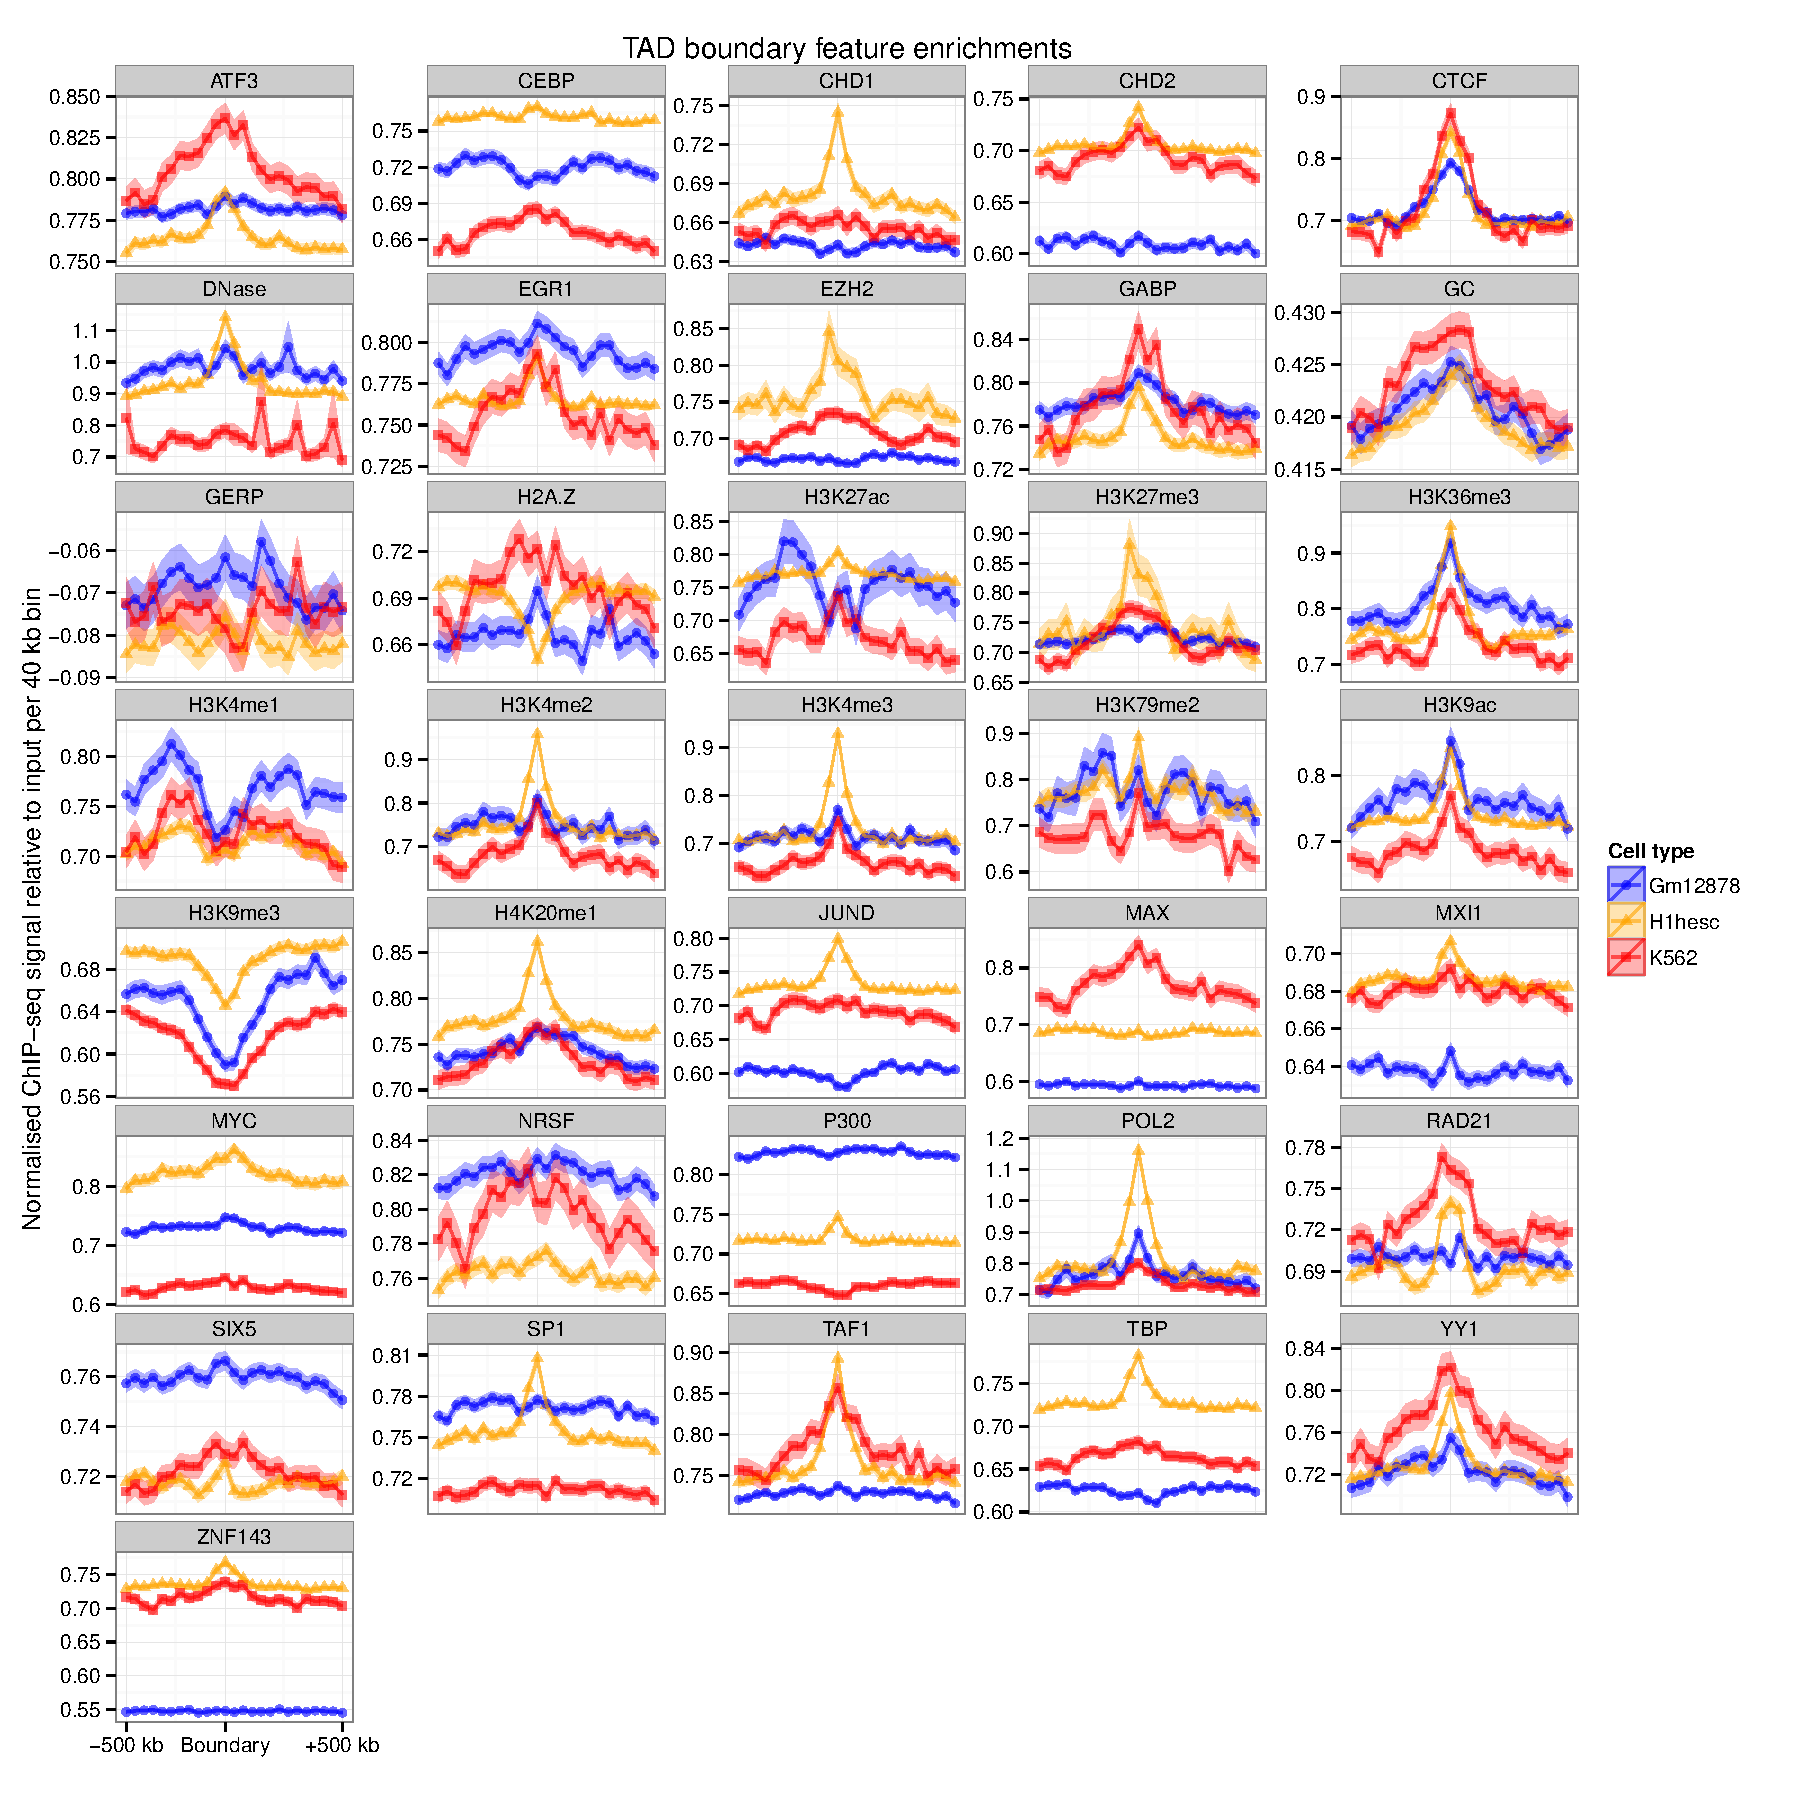
\includegraphics[width=1.12\textwidth]{figs/alltads.pdf}
\captionsetup{width=\textwidth}
\caption{ {\bf Spectra of TAD boundary enrichments and depletions.}
Placeholder
}\label{fig:alltads}
\end{center}
\end{figure} 

\begin{figure}
\begin{center} 
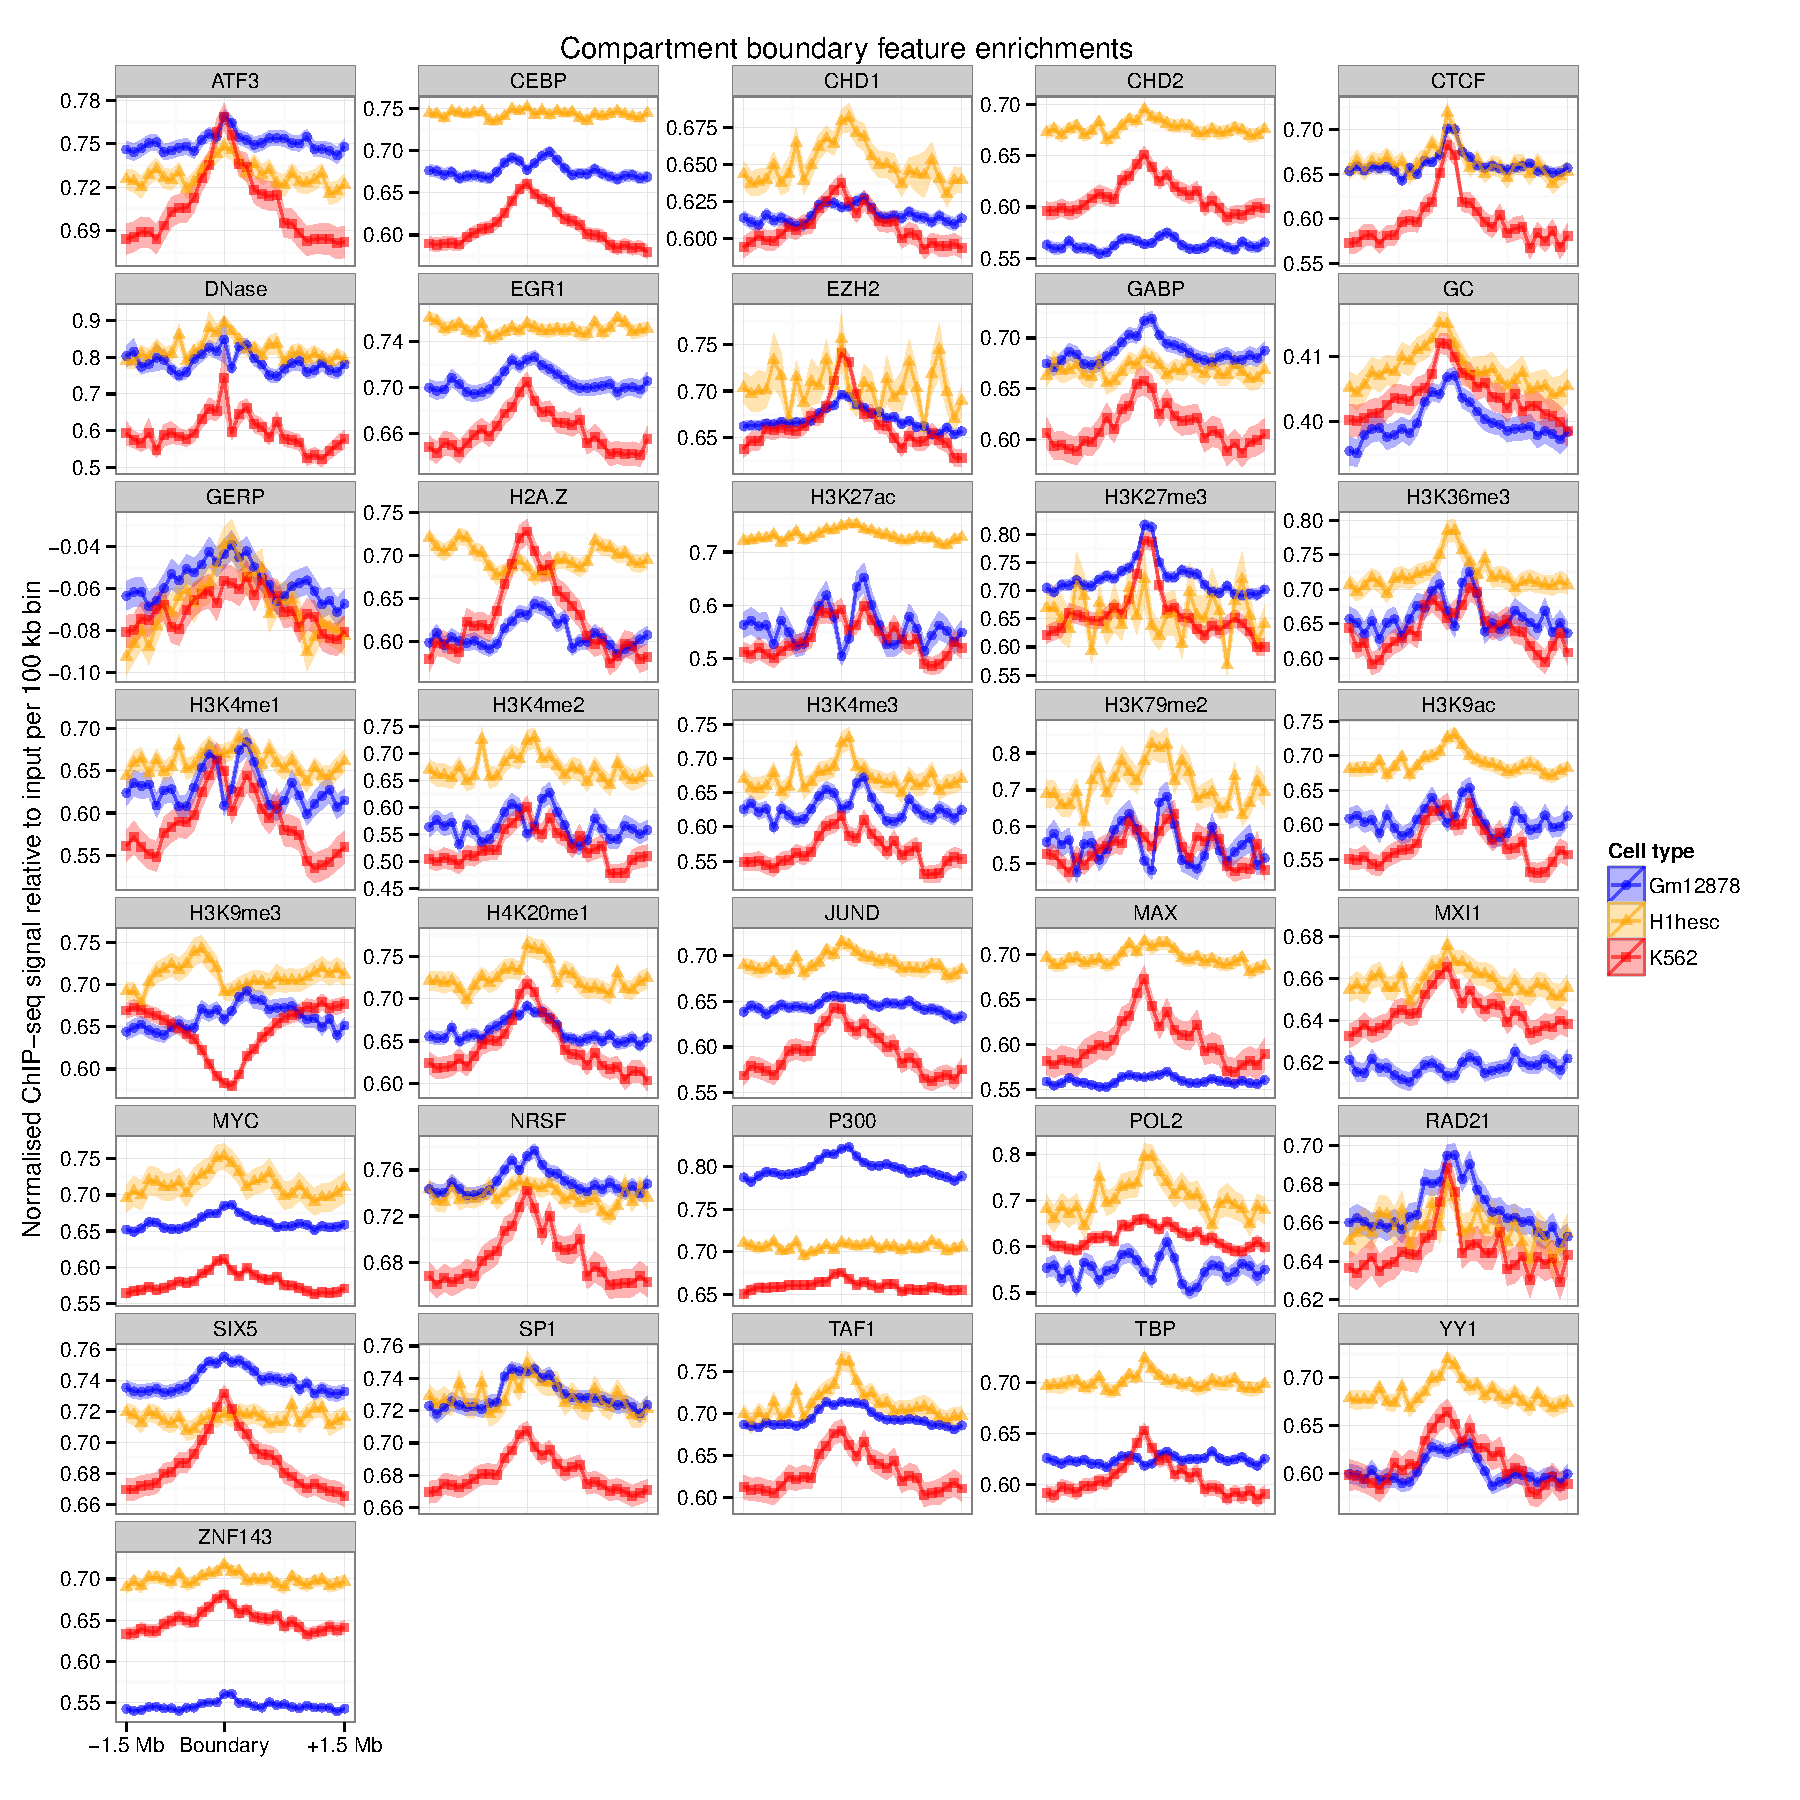
\includegraphics[width=1.12\textwidth]{figs/allcompartments.pdf}
\captionsetup{width=\textwidth}
\caption{ {\bf Spectra of compartment boundary enrichments and depletions.}
Placeholder
}\label{fig:allcompartments}
\end{center}
\end{figure} 

Our findings confirmed the previously reported peaks (CTCF and POL2) and dip (H3K9me3) in ESC data, but also revealed substantial heterogeneity between cell types. CTCF binding was found enriched at TAD boundaries across all cell types, but other features, including H3K36me3 and H3K4me3, show dramatic peaks of enrichment in H1 hESC cells that are not seen consistently in other cell types (Figure 6, Additional file 1: Figure S12). Although the dip in H3K9me3 at TAD boundaries is seen in all cell types, the extent of the depletion varies and is weakest in H1 hESC cells. Many other features show significant, though often modest, enrichments in a particular cell type. However, overall the complexity of TAD boundaries (measured as the number of strongly enriched features) is notably higher in H1 hESC than in the other two, more differentiated, cell types (Figure 6), involving large increases in the binding of sequence specific factors such as SP1 and JUND.

\begin{figure}
\begin{center} 
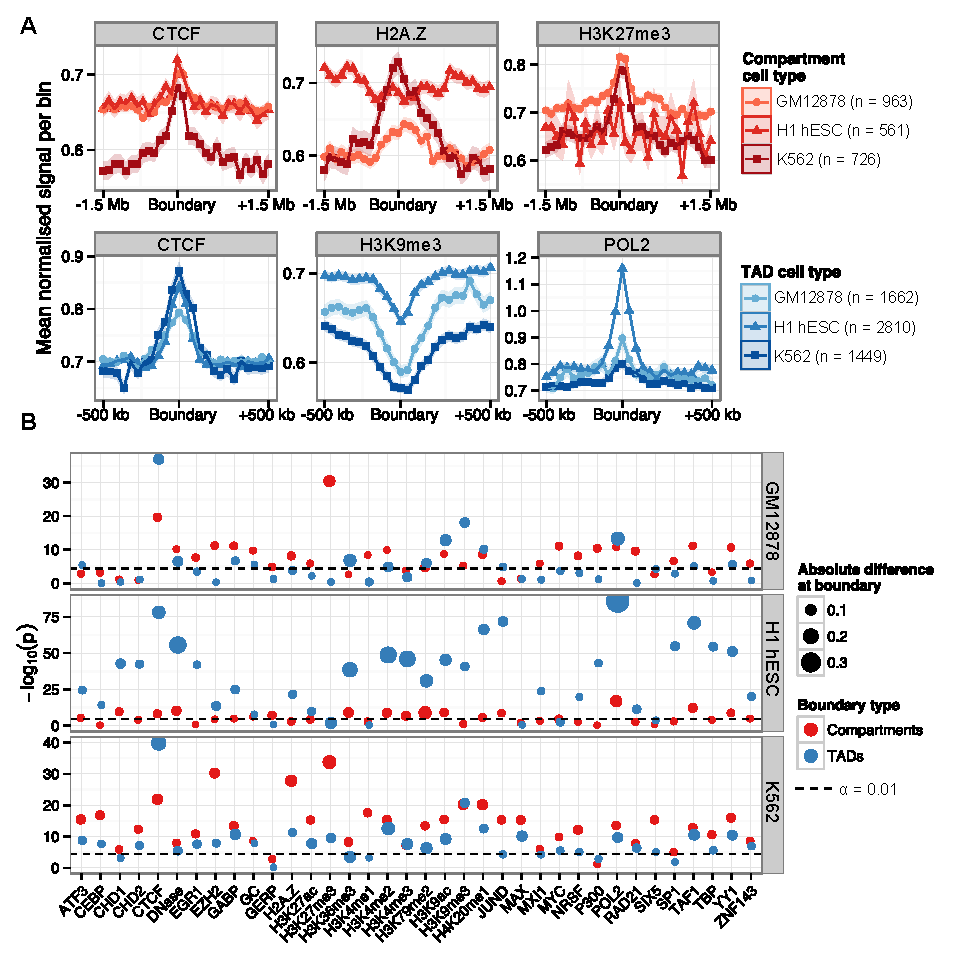
\includegraphics[width=\textwidth]{figs/boundarysummary.pdf}
\captionsetup{width=\textwidth}
\caption{ {\bf Compartment and TAD boundary enrichment summary in three human cell types.}
Placeholder
}\label{fig:boundarysummary}
\end{center}
\end{figure} 

Across all three cell types several features demonstrate consistent
and statistically significant patterns at TAD boundaries (Figure 6,
Figure S12), including peaks associated with active transcription of
genes (POL2, H3K9ac) and dips in H3K9me3, as previously reported.\cite{Dixon2012} However other novel feature peaks of interest emerge
across cell types, such as peaks of H4K20me1, a modification
previously implicated in chromatin compaction.\cite{Evertts2013} We also observe consistent increases in GC content at TAD boundaries, at a scale that is difficult to reconcile with the presence of smaller-scale features such as repeat elements or CpG islands (Additional file 1: Figure S12).

Where neighbouring genomic regions occupy contrasting A and B nuclear
compartments, the disparity implies the presence of a boundary
region. Putative compartment boundaries were identified by using an
HMM to infer the state sequence of A/B compartments across the genome
based on observed principal component eigenvectors. Analogously to the
TAD boundary analysis we then sought significant enrichments or
depletions in 36 chromatin features over these compartment boundaries
(Figure 6, Figure S13).  Compartment boundaries display similar
spectra of enrichments to previously studied TAD boundaries
\cite{Dixon2012} but at lower resolution, reflecting the different
scales of these levels of organization (Figure 6B, Figure S13). Peaks
associated with active promoters (POL2, TAF1, H3K9ac) are again
evident. Parallel enrichments of CTCF, YY1 and H4K20me1 are also seen
at compartment boundaries, as they were for TAD boundaries, in each
cell type under study. In addition, compartment boundaries show
enrichments of H3K79me2, which is known to play critical roles in
cellular reprogramming.\cite{Onder2012} Remarkably, H3K79me2 has
also recently been shown to mark the borders of small (hundreds of bp)
regions of open chromatin.\cite{Chai2013} Thus there may be
similarities in chromatin compaction boundaries at very different
scales.

Certain features show intriguing contrasts between cell types the
histone variant H2A.Z lacks any trace of enrichment at H1 hESC
compartment boundaries, but is significantly enriched in the other two
cell types (Figure 6A), consistent with reports describing H2A.Z
relocation during cellular differentiation.\cite{Ku2012} Compartment
boundaries also show enrichment for the cohesin complex subunit RAD21
in the two hematopoietic cell types , and cohesin is
another factor implicated in modulating nuclear architecture in
partnership with CTCF.\cite{Zuin2013} Various other enrichments
with very modest effect sizes are also evident at compartment
boundaries (Figure 6B, Figure S13). In contrast to TAD boundaries, the
composition of compartment boundaries appears least complex in H1
hESC, relative to the other two cell types. Overall compartment and
TAD boundaries are associated with overlapping spectra of chromatin
features across cell types. These involve DNA binding proteins
implicated in chromosome architecture (CTCF, YY1, RAD21), but also
implicate the initiation and repression of transcription as critical
to boundary formation. However these two boundary classes occur at
different scales, with patterns of informative features typically
spanning regions up to 500 Kb for TAD boundaries, and patterns
associated with compartment boundaries often spanning more than 1 Mb.

\subsection{CTCF and YY1}

\begin{figure}
\begin{center} 
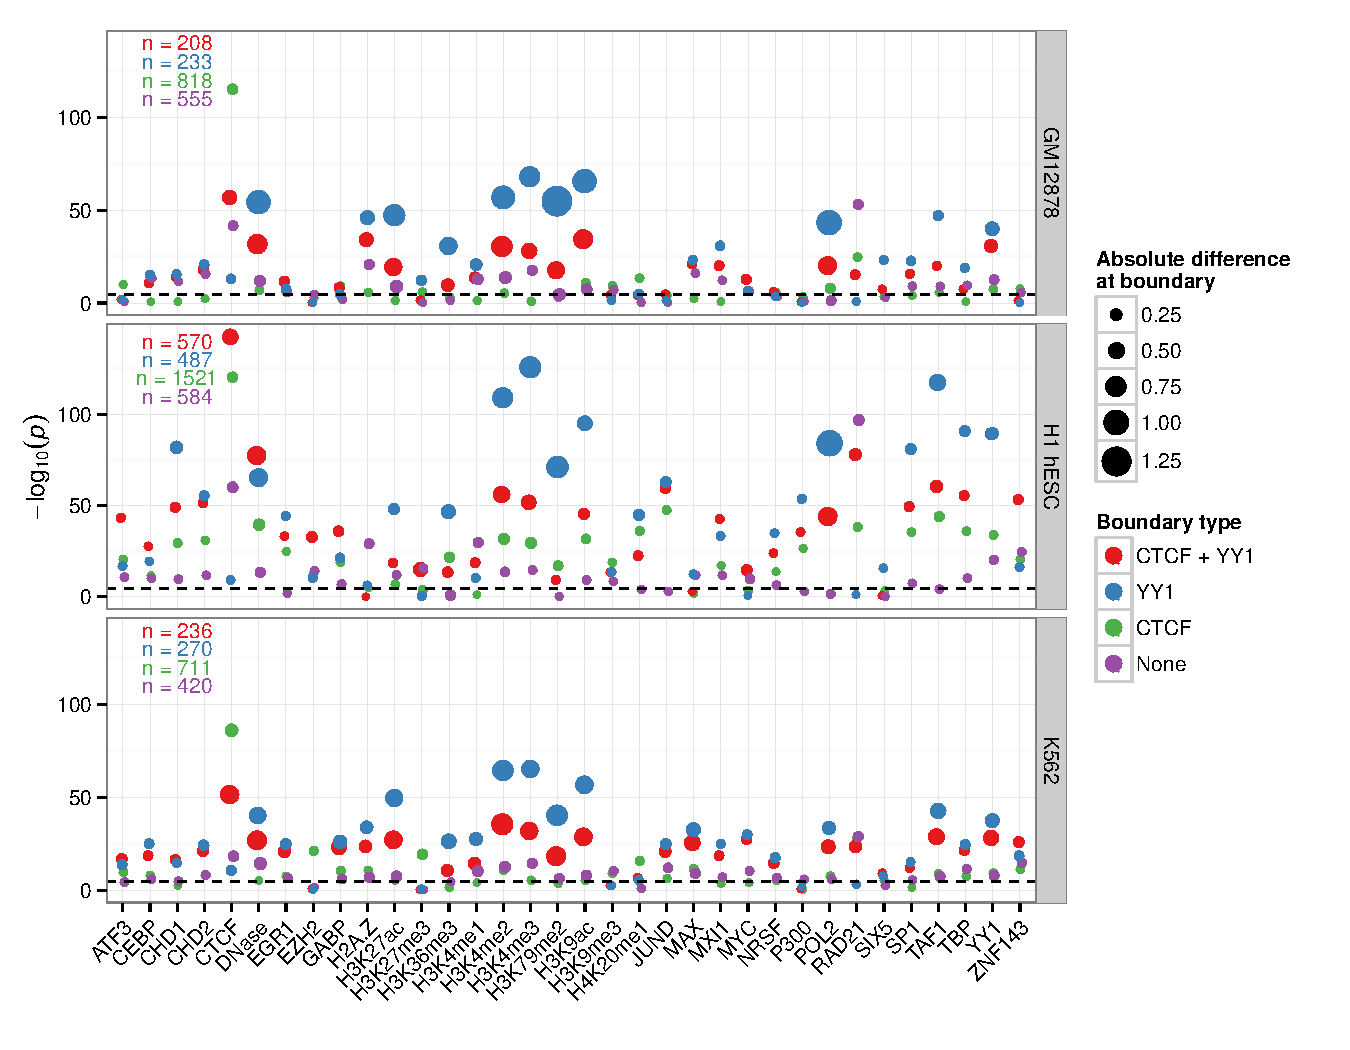
\includegraphics[width=1.2\textwidth]{figs/ctcfyy1.pdf}
\captionsetup{width=\textwidth}
\caption{ {\bf Distinct enrichments of CTCF and YY1 boundaries.}
Placeholder
}\label{fig:ctcfyy1}
\end{center}
\end{figure} 

Significant peaks in YY1 are evident in all cell
types, which is intriguing given the evidence that YY1 and CTCF
cooperate to affect long distance interactions.\cite{Atchison2014} Co-binding of CTCF with YY1 has also been shown
to identify a subset of highly conserved CTCF sites.\cite{Schwalie2013} Co-binding of CTCF and YY1 may also therefore be
a contributing factor in the establishment of TAD boundaries, which
appear to be broadly conserved across mammals.\cite{Dixon2012} To
test this, we split our sets of TAD boundaries into those possessing
ChiP-seq peaks (region peaks called by ENCODE \cite{Dunham2012}) for
CTCF, YY1, both CTCF and YY1 (overlapping peaks) and neither. We then
tested each boundary subset for genome-wide enrichments of the other
features in our dataset (Figure S14). Unexpectedly, we found that
boundaries marked by YY1 (without overlapping CTCF peaks) were
generally most strongly-enriched for other features in our dataset. We
also found that boundaries lacking both CTCF and YY1 peaks showed
instead the strongest enrichments for RAD21 in each cell type (Figure
S14), reinforcing previous findings that describe the distinct
influences of CTCF and cohesin in organizing chromatin structure.\cite{Zuin2013, Seitan2013, Phillips-Cremins2013}

\subsection{Repeats}

% New stuff on repeat classes and boundaries over TAD + compartments, per cell type

\section{De novo boundary prediction}

\section{MetaTAD boundaries}

\section{Other boundaries}

\subsection{Giemsa bands}

\subsection{Superboundaries}

Thus far compartment and TAD boundaries have been considered separately, however it is of interest to consider how these boundary regions interact across scales. Open questions remain about the co-occurence of these two boundary regions, and whether 


\ifstandalone
\begin{small}
\bibliography{/Users/benmoore/Documents/library,/Users/benmoore/Documents/customrefs}
\end{small}
\fi

\end{document}
